 
\chapter{Generalized Linear Models: A Unification}
   \chaptermark{GLM: a Unification}


This chapter unifies Chapters \ref{chapter::binary-logit}--\ref{chapter::count} under the formulation of the generalized linear model (GLM) by \citet{nelder1972generalized}. 



\section{Generalized Linear Models}

So far we have discussed the following models for independent observations
$(y_{i},x_{i})_{i=1}^{n}$.

\begin{example}\label{eg::gaussianlinearmodel}
The Normal linear model for continuous outcomes assumes
\begin{equation}
y_{i}\mid x_{i}\sim\N(\mu_{i},\sigma^{2}),\quad\text{with }\mu_{i}=x_{i}^{\T}\beta.\label{eq:gaussianlinearmodel}
\end{equation}
\end{example}


\begin{example}\label{eg::binarylogisticmodel}
The logistic model for binary outcomes assumes
\begin{equation}
y_{i}\mid x_{i}\sim\textup{Bernoulli}(\mu_{i}),\quad\text{with }\mu_{i}=\frac{e^{x_{i}^{\T}\beta}}{1+e^{x_{i}^{\T}\beta}} . \label{eq:logisticlinearmodel}
\end{equation}
\end{example}


\begin{example}\label{eg::countpoissonmodel}
The Poisson model for count outcomes assumes 
\begin{equation}
y_{i}\mid x_{i}\sim\textup{Poisson}(\mu_{i}),\quad\text{with }\mu_{i}=e^{x_{i}^{\T}\beta} . \label{eq:poissonlinearmodel}
\end{equation}
\end{example}


\begin{example}\label{eg::countnbmodel}
The Negative-Binomial model for overdispersed count outcomes assumes
\begin{equation}
y_{i}\mid x_{i}\sim\textsc{NB}(\mu_{i},\delta),\quad\text{with }\mu_{i}=e^{x_{i}^{\T}\beta} . \label{eq: nblinearmodel}
\end{equation}
We use $\delta$ for the dispersion parameter to avoid
confusion because $\theta$ means something else below (Chapter \ref{chapter::count} uses $\theta$ for the dispersion parameter). 
\end{example}

In the above models, $\mu_i$ denotes the conditional mean. This chapter 
will unify Examples \ref{eg::gaussianlinearmodel}--\ref{eg::countnbmodel} as GLMs. 

\subsection{Exponential family\label{subsec:Exponential-family}}

Consider a general conditional probability density or mass function:
\begin{equation}
f(y_{i}\mid x_{i};\theta_{i},\phi)=\exp\left\{ \frac{y_{i}\theta_{i}-b(\theta_{i})}{a(\phi)}+c(y_{i},\phi)\right\} ,\label{eq:natualexponentialfamily-dispersion}
\end{equation}
where $(\theta_{i},\phi)$ are unknown parameters, and $\left\{ a(\cdot),  b(\cdot),c(\cdot,\cdot)\right\} $
are known functions. The above conditional density (\ref{eq:natualexponentialfamily-dispersion})
is called the {\it natural exponential family with dispersion}, where $\theta_{i}$
is the natural parameter depending on $x_{i}$, and $\phi$ is the
dispersion parameter. Sometimes, $a(\phi)=1$ and $c(y_{i},\phi)=c(y_{i})$,
simplifying the conditional density to a {\it natural exponential family}. Examples \ref{eg::gaussianlinearmodel}--\ref{eg::countnbmodel}
have a unified structure as (\ref{eq:natualexponentialfamily-dispersion}), as detailed below. 

\setcounter{example}{0}
\begin{example}[continued]\label{eg::gaussianlinearmodel-continue}
 Model (\ref{eq:gaussianlinearmodel}) has conditional probability
density function
\begin{align*}
f(y_{i}  \mid x_{i};\mu_{i},\sigma^{2}) &=(2\pi\sigma^{2})^{-1/2}\exp\left\{ -\frac{(y_{i}-\mu_{i})^{2}}{2\sigma^{2}}\right\} \\
 & =\exp\left\{ \frac{y_{i}\mu_{i}-\frac{1}{2}\mu_{i}^{2}}{\sigma^{2}}-\frac{1}{2}\log(2\pi\sigma^{2})-\frac{y_{i}^{2}}{2\sigma^{2}}\right\} ,
\end{align*}
with 
\[
\theta_{i}=\mu_{i},\quad b(\theta_{i})=\frac{1}{2}\theta_{i}^{2},
\]
and
$$
\phi=\sigma^{2},\quad a(\phi)=\sigma^{2} = \phi.
$$ 
\end{example}



\begin{example}[continued]\label{eg::binarylogisticmodel-continue}
 Model (\ref{eq:logisticlinearmodel}) has conditional probability
mass function
\begin{align*}
f(y_{i}  \mid x_{i};\mu_{i}) &=\mu_{i}^{y_{i}}(1-\mu_{i})^{1-y_{i}} \\
&=\left(\frac{\mu_{i}}{1-\mu_{i}}\right)^{y_{i}}(1-\mu_{i})\\
 & =\exp\left\{ y_{i}\log\frac{\mu_{i}}{1-\mu_{i}}-\log\frac{1}{1-\mu_{i}}\right\} ,
\end{align*}
with
\[
\theta_{i}=\log\frac{\mu_{i}}{1-\mu_{i}} \Longleftrightarrow \mu_i = \frac{e^{\theta_{i}}}{1 + e^{\theta_{i}}},
\quad b(\theta_{i})=\log\frac{1}{1-\mu_{i}}=\log(1+e^{\theta_{i}}),
\]
and
$$
 a(\phi)=1.
$$
\end{example}


\begin{example}[continued]\label{eg::countpoissonmodel-continue}
 Model (\ref{eq:poissonlinearmodel}) has conditional probability mass
function
\begin{align*}
f(y_{i}  \mid x_{i};\mu_{i}) &=e^{-\mu_{i}}\frac{\mu_{i}^{y_i}}{y_i!} \\
&  =\exp\left\{ y_{i}\log\mu_{i}-\mu_{i}-\log y_{i}!\right\} ,
\end{align*}
with
\[
\theta_{i}=\log\mu_{i},\quad b(\theta_{i})=\mu_{i}=e^{\theta_{i}},
\]
and
$$
a(\phi)=1.
$$
\end{example}


\begin{example}[continued]\label{eg::countnbmodel-continue}
 Model (\ref{eq: nblinearmodel}), for a {\it fixed} $\delta$, has conditional
probability mass function
\begin{align*}
&f(y_{i}  \mid x_{i};\mu_{i})  \\
& =\frac{\Gamma(y_{i}+\delta)}{\Gamma(\delta )\Gamma(y_{i}+1)}\left(\frac{\mu_{i}}{\mu_{i}+\delta}\right)^{y_{i}}\left(\frac{\delta}{\mu_{i}+\delta}\right)^{\delta}\\
 & =\exp\left\{ y_{i}\log\frac{\mu_{i}}{\mu_{i}+\delta}-\delta\log\frac{\mu_{i}+\delta}{\delta}  
  +\log\Gamma(y_{i}+\delta)-\log\Gamma(\delta)-\log\Gamma(y_{i}+1)\right\} ,
\end{align*}
with 
\[
\theta_{i}=\log\frac{\mu_{i}}{\mu_{i}+\delta}  \Longleftrightarrow  \frac{\delta}{  \mu_{i}+\delta  } = 1- e^{\theta_i}  ,
\quad b(\theta_{i})=\delta\log\frac{\mu_{i}+\delta}{\delta}= - \delta\log (1-e^{\theta_{i}}) ,
\]
and
$$
 a(\phi)=1.
$$
\end{example}



 

The logistic and Poisson models are simpler without the dispersion parameter.
The Normal linear model has a dispersion parameter for the variance.
The Negative-Binomial model is more complex: without fixing $\delta$
it does not belong to the exponential family with dispersion. 

The exponential family (\ref{eq:natualexponentialfamily-dispersion})
has nice properties derived from the classic Bartlett's identities \citep{bartlett1953approximate}.
I first review Bartlett's identities:
\begin{lemma}
\label{lemma:bartlett-identity}Given a probability density or mass
function $f(y\mid\theta)$ indexed by a scalar parameter $\theta$, if we can
change the order of expectation and differentiation, then
$$
E\left(\frac{\partial\log f(y\mid\theta)}{\partial\theta}\right)=0
$$
and
$$
E\left\{ \left(\frac{\partial\log f(y\mid\theta)}{\partial\theta}\right)^{2}\right\} =E\left(-\frac{\partial^{2}\log f(y\mid\theta)}{\partial\theta^{2}}\right).
$$
\end{lemma}

This lemma is well-known in classic statistical theory for likelihood,
and I give a simple proof below.

\begin{myproof}{Lemma}{\ref{lemma:bartlett-identity}}
Define $\ell (y\mid \theta) = \log f(y\mid \theta)$ as the log likelihood function, so $e^{\ell (y\mid \theta)}$ is the density satisfying 
$$
\int e^{\ell (y\mid \theta)} \d y  = \int f(y\mid \theta)\d y = 1
$$
by the definition of a probability density function (we can replace the integral by summation for a probability mass function). Differentiate the above identity to obtain
\begin{eqnarray*}
&& \frac{\partial }{\partial \theta} \int e^{\ell (y\mid \theta)} \d y = 0 \\
 &\Longrightarrow  &   \int  \frac{\partial }{\partial \theta} e^{\ell (y\mid \theta)} \d y = 0 \\
 & \Longrightarrow  &   \int  e^{\ell (y\mid \theta)} \frac{\partial }{\partial \theta} \ell (y\mid \theta)  \d y = 0 ,
%  & \Longrightarrow  &    E\left\{  \frac{ \partial  \ell (y\mid \theta)  }{ \partial \theta }  \right\} =0  . 
\end{eqnarray*}
which implies Bartlett's first identity. 
Differentiate it twice to obtain
\begin{eqnarray*}
&& \frac{\partial }{\partial \theta}  \int  e^{\ell (y\mid \theta)} \frac{\partial }{\partial \theta} \ell (y\mid \theta)  \d y = 0 \\
&\Longrightarrow &  \int  \left[ e^{\ell (y\mid \theta)} \left\{ \frac{\partial }{\partial \theta} \ell (y\mid \theta) \right\}^2  
+e^{\ell (y\mid \theta)} \frac{\partial^2 }{\partial \theta^2} \ell (y\mid \theta) \right] 
   \d y = 0 ,
%&\Longrightarrow &    E\left\{ \left(\frac{\partial\log f(y\mid\theta)}{\partial\theta}\right)^{2}\right\} =E\left(-\frac{\partial^{2}\log f(y\mid\theta)}{\partial\theta^{2}}\right).
\end{eqnarray*}
which implies Bartlett's second identity. 
\end{myproof}




Lemma \ref{lemma:bartlett-identity}
implies the moments of the exponential family (\ref{eq:natualexponentialfamily-dispersion}).
\begin{theorem}
\label{theorem:The-first-two-moments-NEF}The first two moments of (\ref{eq:natualexponentialfamily-dispersion})
are
$$
E(y_{i}\mid x_{i};\theta_{i},\phi)\equiv\mu_{i}=b'(\theta_{i})
$$
and
$$
\var(y_{i}\mid x_{i};\theta_{i},\phi)\equiv\sigma_{i}^{2}=b''(\theta_{i})a(\phi).
$$ 
\end{theorem}



\begin{myproof}{Theorem}{\ref{theorem:The-first-two-moments-NEF}}
The first two derivatives of the log conditional density are
\[
\frac{\partial\log f(y_{i}\mid x_{i};\theta_{i},\phi)}{\partial\theta_{i}}=\frac{y_{i}-b'(\theta_{i})}{a(\phi)},\quad\frac{\partial^{2}\log f(y_{i}\mid x_{i};\theta_{i},\phi)}{\partial\theta_{i}^{2}}=-\frac{b''(\theta_{i})}{a(\phi)}.
\]
Lemma \ref{lemma:bartlett-identity} implies that
\[
E\left\{ \frac{y_{i}-b'(\theta_{i})}{a(\phi)}\right\} =0,\quad E\left[\left\{ \frac{y_{i}-b'(\theta_{i})}{a(\phi)}\right\} ^{2}\right]=\frac{b''(\theta_{i})}{a(\phi)},
\]
which further imply the first two moments of $y_{i}$ given $x_i$. 
\end{myproof}


\subsection{Generalized linear model}

Section \ref{subsec:Exponential-family} is general, allowing the
mean parameter $\mu_{i}$ to depend on $x_{i}$ in an arbitrary way.
This flexibility does not immediately generate a useful statistical
procedure. To borrow information across observations, we assume that
the relationship between $y_{i}$ and $x_{i}$ remain ``stable'' and
can be captured by a fixed parameter $\beta$. A simple starting point
is to use $x_{i}^{\T}\beta$ to approximate $\mu_{i}$, which, however,
works naturally only for outcomes taking values in a wide range of $(-\infty, \infty)$. For general outcome variables,
we can link its mean and the linear combination of covariates by
\[
\mu_{i}=\mu(x_{i}^{\T}\beta),
\]
where $\mu(\cdot)$ is a known function and $\beta$ is an unknown
parameter. The inverse of $\mu(\cdot)$ is called the link function. This is called a GLM, which
has the following components:
\begin{enumerate}
[(C1)]
\item the conditional distribution (\ref{eq:natualexponentialfamily-dispersion})
as an exponential family with dispersion;
\item the conditional mean $\mu_{i}=b'(\theta_{i})$ and variance $\sigma_{i}^{2}=b''(\theta_{i})a(\phi)$
in Theorem \ref{theorem:The-first-two-moments-NEF};
\item the function linking the conditional mean and covariates $\mu_{i}=\mu(x_{i}^{\T}\beta)$. 
\end{enumerate}
Models (\ref{eq:gaussianlinearmodel})--(\ref{eq: nblinearmodel})
are the classical examples. 
Figure \ref{fig:Quantities-in-a-glm} illustrates the relationship among key quantities in a GLM.  In particular,
\begin{equation}
\theta_{i}=(b')^{-1}(\mu_{i})=(b')^{-1}\left\{ \mu(x_{i}^{\T}\beta)\right\} \label{eq:theta-beta-link}
\end{equation}
depends on $x_i$ and $\beta$, with $(b')^{-1}$ indicating the inverse function of $b'(\cdot)$. 



\begin{figure}[ht]
\centering 
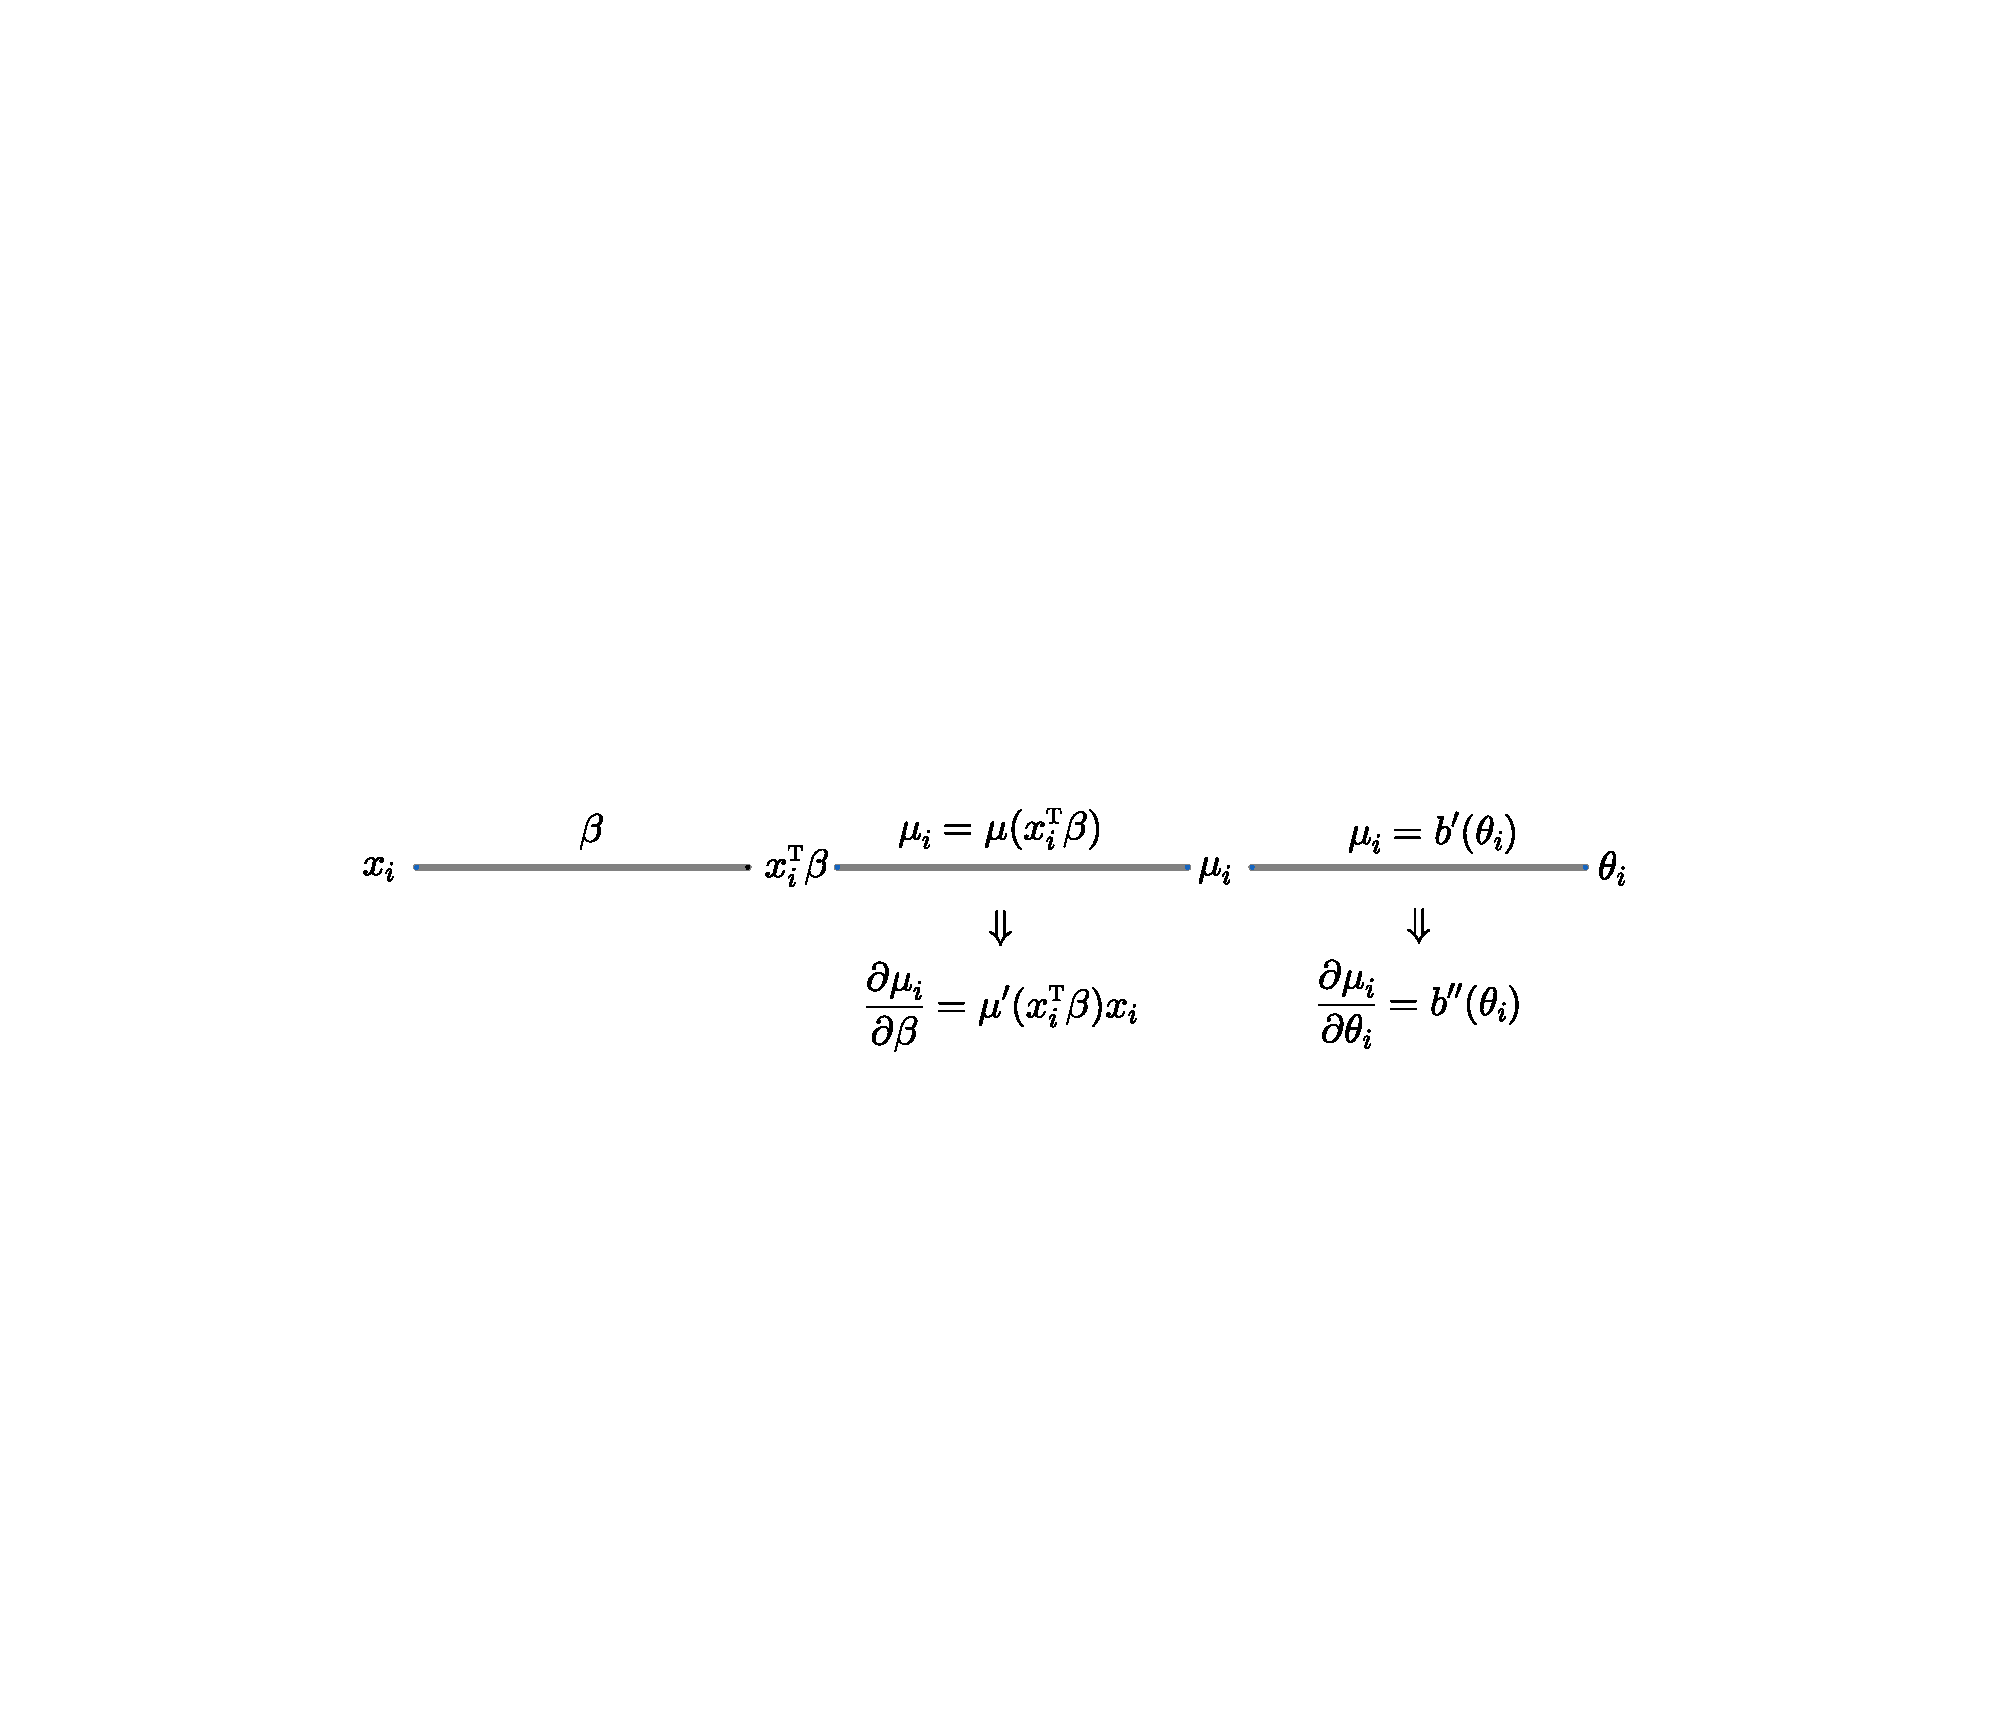
\includegraphics[width = \textwidth]{figures/nef-glm-plot}
\caption{Quantities in a GLM\label{fig:Quantities-in-a-glm}}
\end{figure}



\section{MLE for GLM}\label{sec::mle-glm-fisher}

The contribution of unit $i$ to the log-likelihood function is
\[
\ell_{i}=\log f(y_{i}\mid x_{i};\beta,\phi)=\frac{y_{i}\theta_{i}-b(\theta_{i})}{a(\phi)}+c(y_{i},\phi).
\]
The  contribution of unit $i$ to the score function is
\[
\frac{\partial\ell_{i}}{\partial\beta}=\frac{\partial\ell_{i}}{\partial\theta_{i}}\frac{\partial\theta_{i}}{\partial\mu_{i}}\frac{\partial\mu_{i}}{\partial\beta},
\]
where 
\begin{align*}
\frac{\partial\ell_{i}}{\partial\theta_{i}} & =\frac{y_{i}-b'(\theta_{i})}{a(\phi)},\\
\frac{\partial\theta_{i}}{\partial\mu_{i}} & =\frac{1}{b''(\theta_{i})}=\frac{a(\phi)}{\sigma_{i}^{2}}
\end{align*}
follow from Theorem \ref{theorem:The-first-two-moments-NEF}. 
So 
\[
\frac{\partial\ell_{i}}{\partial\beta}=\frac{y_{i}-b'(\theta_{i})}{\sigma_{i}^{2}}\frac{\partial\mu_{i}}{\partial\beta}=\frac{y_{i}-\mu_{i}}{\sigma_{i}^{2}}\frac{\partial\mu_{i}}{\partial\beta},
\]
leading to the following score equation for the MLE:
\begin{equation}
\sumn\frac{y_{i}-\mu_{i}}{\sigma_{i}^{2}}\frac{\partial\mu_{i}}{\partial\beta}=0,\label{eq:score-equation-mle-form1}
\end{equation}
or, more explicitly, 
\[
\sumn\frac{y_{i}-\mu (x_{i}^{\T}\beta) }{\sigma_{i}^{2}}\mu'(x_{i}^{\T}\beta)x_{i}=0
\]

The general relationship (\ref{eq:theta-beta-link}) between $\theta_{i}$
and $\beta$ is quite complicated. A natural choice of $\mu(\cdot)$
is to cancel $(b')^{-1}$ in \eqref{eq:theta-beta-link} so that 
\[
\mu(\cdot)=b'(\cdot)\Longrightarrow\theta_{i}=x_{i}^{\T}\beta.
\]
This link function $\mu(\cdot)$ is called the canonical link or the natural link, which leads
to further simplifications:
\begin{align*}
\mu_{i} & =b'(x_{i}^{\T}\beta)\Longrightarrow\frac{\partial\mu_{i}}{\partial\beta}=b''(x_{i}^{\T}\beta)x_{i}
= b''( \theta_i )x_{i}
=\frac{\sigma_{i}^{2}}{a(\phi)}x_{i},
\end{align*}
and 
\begin{eqnarray}
&&\frac{\partial\ell_{i}}{\partial\beta} = \frac{y_{i}-\mu_{i}}{\sigma_{i}^{2}}\frac{\sigma_{i}^{2}}{a(\phi)}x_{i} 
= a(\phi)^{-1} x_i (y_{i}-\mu_{i}) \nonumber  \\
& \Longrightarrow &
a(\phi)^{-1} \sumn  x_i (y_{i}-\mu_{i})    =0 \nonumber  \\
&\Longrightarrow &  \sumn x_{i}\left(y_{i}-\mu_{i}\right)=0.\label{eq:NormalEquation-NEF-GLM}
\end{eqnarray} 
We have shown that the MLEs of models (\ref{eq:gaussianlinearmodel})--(\ref{eq:poissonlinearmodel})
all satisfy (\ref{eq:NormalEquation-NEF-GLM}). However, the MLE of (\ref{eq: nblinearmodel})
does not because it does not use the natural link function resulting in $\mu(\cdot) \neq b'(\cdot) $: 
$$
\mu(*) = e^{*},\quad 
b'(*) = \delta \frac{e^*}{ 1 - e^*}. 
$$


 
Using Bartlett's second identity in Lemma \ref{lemma:bartlett-identity},
we can write the expected Fisher information conditional on covariates
as
\begin{align*}
\sumn E\left(\frac{\partial\ell_{i}}{\partial\beta}\frac{\partial\ell_{i}}{\partial\beta^{\T}}\mid x_{i}\right) & =\sumn E\left\{ \left(\frac{y_{i}-\mu_{i}}{\sigma_{i}^{2}}\right)^{2}\frac{\partial\mu_{i}}{\partial\beta}\frac{\partial\mu_{i}}{\partial\beta^{\T}}\mid x_{i}\right\} \\
 & =\sumn\frac{1}{\sigma_{i}^{2}}\frac{\partial\mu_{i}}{\partial\beta}\frac{\partial\mu_{i}}{\partial\beta^{\T}}\\
 & =\sumn\frac{1}{\sigma_{i}^{2}}\left\{ \mu'(x_{i}^{\T}\beta)\right\} ^{2}x_{i}x_{i}^{\T}\\
 & =X^{\T}WX,
\end{align*}
where 
\[
W=\text{diag}\left\{ \frac{1}{\sigma_{i}^{2}}\left\{ \mu'(x_{i}^{\T}\beta)\right\} ^{2}\right\} _{i=1}^{n}.
\]
With the canonical link, it further simplifies to
\begin{align*}
\sumn E\left(\frac{\partial\ell_{i}}{\partial\beta}\frac{\partial\ell_{i}}{\partial\beta^{\T}}\mid x_{i}\right) & =\sumn E\left\{ \left(\frac{y_{i}-\mu_{i}}{a(\phi)}\right)^{2}x_{i}x_{i}^{\T}\mid x_{i}\right\} \\
 & =\left\{ a(\phi)\right\} ^{-2}\sumn\sigma_{i}^{2}x_{i}x_{i}^{\T} . 
\end{align*}

We can obtain the estimated covariance matrix by replacing the unknown parameters with their estimates. 
Now we review the estimated covariance matrices of the classical GLMs with canonical links. 
\setcounter{example}{0}
\begin{example}[continued]\label{eg::gaussianlinearmodel-continue1}
In the Normal linear model,  
$
\hat{V} =  \hat{\sigma}^2 (X^{\T} X)^{-1}
$
with $ \sigma^2$ estimated further by the residual sum of squares. 
\end{example}



\begin{example}[continued]\label{eg::binarylogisticmodel-continue1}
In the binary logistic model,  
$
\hat{V} = (X^{\T} \hat{W} X)^{-1}
$
with  $\hat{W}= \text{diag}\{ \hat{\pi}_i (1-\hat{\pi}_i) \}_{i=1}^n $, where $ \hat{\pi}_i  = e^{x_i^{\T} \hat{\beta}} / (1+e^{x_i^{\T} \hat{\beta}}).$
\end{example}


\begin{example}[continued]\label{eg::countpoissonmodel-continue1}
In the Poisson model,  
$
\hat{V} = (X^{\T} \hat{W} X)^{-1}
$
with  $\hat{W}= \text{diag}\{ \hat{\lambda}_i   \}_{i=1}^n $, where $\hat{\lambda}_i  = e^{x_i^{\T} \hat{\beta}}.$
\end{example}


I relegate the derivation of the formula for the Negative-Binomial regression as Problem \ref{hw20::nb-sandwich}. It is a purely theoretical exercise since $\delta$ is usually unknown in practice.


\section{Other GLMs}


The \ri{glm} function in \ri{R} allows for the specification of the \ri{family} parameters, with the corresponding canonical link functions shown below: 
\begin{lstlisting}
binomial(link = "logit")
gaussian(link = "identity")
Gamma(link = "inverse")
inverse.gaussian(link = "1/mu^2")
poisson(link = "log")
quasi(link = "identity", variance = "constant")
quasibinomial(link = "logit")
quasipoisson(link = "log")
\end{lstlisting}
Examples \ref{eg::gaussianlinearmodel-continue1}--\ref{eg::countpoissonmodel-continue1} correspond to the second, the first, and the fifth choices above. Below I will briefly discuss the third choice for the Gamma regression and omit the discussion of other choices. See the help file of the \ri{glm} function and \citet{mccullagh1989generalized} for more details. 


The Gamma$(\alpha, \beta)$ random variable is positive with mean $\alpha/\beta$ and variance $\alpha/\beta^2$. For convenience in modeling, we use a reparametrization Gamma$'(\mu, \nu)$ where  
$$
\begin{pmatrix}
\mu \\
\nu
\end{pmatrix}
= \begin{pmatrix}
\alpha/\beta \\
\alpha 
\end{pmatrix}
\Longleftrightarrow
\begin{pmatrix}
\alpha \\
\beta
\end{pmatrix}
= \begin{pmatrix}
\nu\\
\nu / \mu 
\end{pmatrix}.
$$
So its mean equals $\mu$ and its variance equals $\mu^2 / \nu$ which is quadratic in $\mu$. A feature of the Gamma random variable is that its coefficient of variation equals $1 /  \sqrt{\nu}$ which does not depend on the mean. So  Gamma$'(\mu, \nu)$ is a parametrization based on the mean and the coefficient of variation \citep{mccullagh1989generalized}.\footnote{The coefficient of variation of a random variable $A$ equals  $\sqrt{\var(A)} / E(A)$. } 
Gamma$'(\mu, \nu)$ has density
$$
f(y)  =  \frac{\beta^\alpha }{ \Gamma (\alpha) } y^{\alpha - 1} e^{- \beta y} 
=  \frac{ (\nu / \mu )^\nu }{ \Gamma (\nu) } y^{\nu - 1} e^{- (\nu / \mu ) y} ,
$$ 
and we can verify that it belongs to the exponential family with dispersion. 
Gamma regression assumes
$$
y_i \mid x_i \sim \text{Gamma}' (\mu_i, \nu)
$$
where $\mu_i = e^{x_i^{\T} \beta}$. So it is also a log-linear model. This does not correspond to the canonical link. Instead, we should specify \ri{Gamma(link = "log")} to fit the log-linear Gamma regression model. 

The log-likelihood function is
$$
\log L(\beta, \nu) = 
\sumn \left\{ 
- \frac{  \nu y_i }{  e^{x_i^{\T} \beta} }  + (\nu - 1)\log y_i + \nu \log \nu - \nu x_i^{\T} \beta - \log\Gamma(\nu)
\right\} .
$$
Then
$$
\frac{ \partial  \log L(\beta, \nu) }{\partial \beta } = 
\sumn ( \nu y_i e^{ - x_i^{\T} \beta}  x_i  - \nu x_i ) = 
\nu \sumn e^{ - x_i^{\T} \beta}  (y_i -  e^{x_i^{\T} \beta}) x_i  
$$
and
$$
\frac{ \partial^2  \log L(\beta, \nu) }{\partial \beta \partial \nu } =
 \sumn e^{ - x_i^{\T} \beta}  (y_i -  e^{x_i^{\T} \beta}) x_i  .
$$
So the MLE for $\beta$ solves the following estimating equation
$$
\sumn e^{ - x_i^{\T} \beta}  (y_i -  e^{x_i^{\T} \beta}) x_i   = 0.
$$
Moreover,  $ \partial^2  \log L(\beta, \nu)  / \partial \beta \partial \nu  $ has expectation zero
so the Fisher information matrix is diagonal. In fact, it is identically zero when evaluated at $\hat\beta$ since it is identical to the estimating equation. 

I end this subsection with a comment on the estimating equation of $\beta$. It is similar to the Poisson score equation except for the additional weight $e^{ - x_i^{\T} \beta} $. For positive outcomes, it is also conventional to fit OLS of $\log y_i$ on $x_i$, resulting in the following estimating equation
$$
\sumn    (\log y_i - x_i^{\T} \beta) x_i   = 0.
$$
\citet{firth1988multiplicative} compared  Gamma and log-Normal regressions based on efficiency. However, these two models are not entirely comparable: Gamma regression assumes that the log of the conditional mean of $y_i$ given $x_i$ is linear in $x_i$, whereas log-Normal regression assumes that the conditional mean of $\log y_i$ given $x_i$ is linear in $x_i$. By Jensen's inequality, $\log E(y_i\mid x_i)   \geq  E( \log y_i\mid x_i)  .$
See Problem \ref{hw20::gamma-regression} for more discussions of Gamma regression. 



 




\section{Homework problems}

 

\paragraph{MLE in GLMs with binary regressors}\label{hw20::mle-binary-z}

The MLEs for $\beta$ in Models (\ref{eq:gaussianlinearmodel})--(\ref{eq:poissonlinearmodel})
do not have explicit formulas in general. But in the special case
with the covariate $x_{i}$ containing $1$ and a binary covariate $z_i \in \{0, 1\}$, their
MLEs do have simple formulas. Find them in terms of sample means of the outcomes.


Then find the variance estimators of $\hat\beta$. 



 
\paragraph{Negative-Binomial covariance matrices}\label{hw20::nb-sandwich}

Assume that $\delta$ is known. 
Derive the estimated asymptotic covariance matrices of the MLE in the Negative-Binomial regression with $\mu_i = e^{x_i^{\T} \beta}$.



\paragraph{Gamma regression}
\label{hw20::gamma-regression}

Verify that Gamma$'(\mu, \nu)$ belongs to the natural exponential family with dispersion. Derive the first- and second-order derivatives of the log-likelihood function and Newton's algorithm for computing the MLE. 
Derive the estimated asymptotic covariance matrices of the MLE. 


Show that if $y_i \mid x_i \sim $ Gamma$'(\mu_i, \nu)$ with $\mu_i = e^{x_i^{\T} \beta}$, then
$$
E(\log y_i \mid x_i ) = \psi(\nu) - \log (\nu) + x_i^{\T} \beta
$$
and
$$
\var(\log y_i \mid x_i ) = \psi'(\nu)
$$
where $\psi(\nu) = \diff \log  \Gamma  (\nu) / \diff \nu$ is the digamma function and $\psi'(\nu)$ is the trigamma function. 



Remark: Use Proposition \ref{thm:gammamoments-log} to calculate the moments.  The above conditional mean function ensures that the OLS estimator of $\log y_i$ on $x_i$ is consistent for all components of $\beta$ except for the intercept. 




 
